\documentclass[tikz, border=10pt]{standalone}

\begin{document}
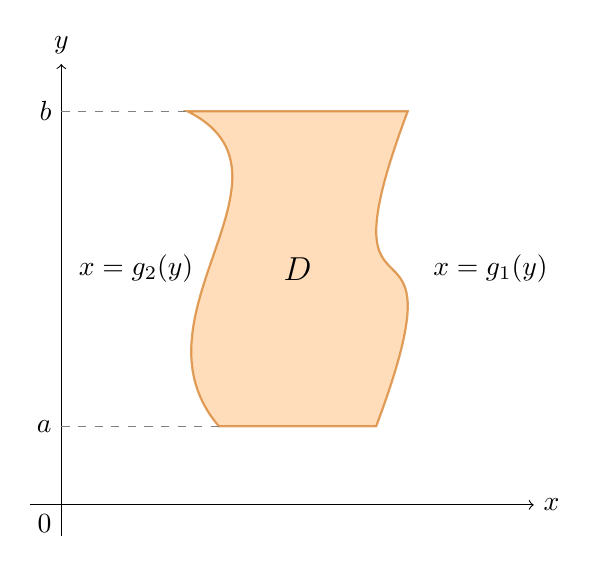
\begin{tikzpicture}[scale=2]
    % Type II (rotated) region: x between functions of y, y in [a,b]
    \def\ya{0.5}
    \def\yb{2.5}
    \def\xmax{3}

    % sample coordinates for left/right curves (as functions of y)
    \coordinate (L1) at (1,\ya);
    \coordinate (L2) at (0.8,\yb);
    \coordinate (R1) at (2.0,\ya);
    \coordinate (R2) at (2.2,\yb);

    % fill the type II region (x between two curves for y in [a,b])
    \draw[orange!80!black, thick, fill=orange!45, opacity=0.6]
        (L1) .. controls (0.4,1.2) and (1.6,2.1) .. (L2) --
        (R2) .. controls (1.6,0.9) and (2.6,2.1) .. (R1) -- cycle;

    % axes (y horizontal, x vertical style visually emphasized)
    \draw[->] (-0.2, 0) -- (\xmax, 0) node[right] {$x$};
    \draw[->] (0, -0.2) -- (0, \yb+0.3) node[above] {$y$};
    \node[below left] at (0,0) {$0$};

    % dashed horizontal (constant-y) lines marking y=a and y=b
    \draw[dashed, gray] (0,\ya) -- (L1);
    \draw[dashed, gray] (0,\yb) -- (L2);

    % labels on the y-axis for a and b
    \node[left] at (0,\ya) {$a$};
    \node[left] at (0,\yb) {$b$};

    % label the boundary curves as functions x = g_1(y), x = g_2(y)
    \node[left] at (0.9,1.5) {$x=g_2(y)$};
    \node[right] at (2.3,1.5) {$x=g_1(y)$};

    % region label
    \node[font=\large] at (1.5,1.5) {$D$};
\end{tikzpicture}
\end{document}
